\chapter{Concept}
The application should be accessible to all employees of SinnerSchrader. Due to the heterogeneity of the people’s computer setups running Windows, macOS and Linux, creating a native application supported by everyone’s system is a rather complicated task. A web application using standard technologies does not only solve this problem, but can also be used from mobile devices such as smart phones and tablets. Furthermore, there is no need to manually install and update the software so that it can be assumed that all users use the latest version of the application. This is not only a positive factor regarding the overall usability of the system, but also assures bugs and security issues are eliminated the moment a fixed version of the software is deployed. All those advantages compared to native clients and the fact that SinnerSchrader’s expertise lies in the development of web applications made the decision that this tool should be realized as such. (TODO: wording as such)

\begin{figure}[h]
    \centering
    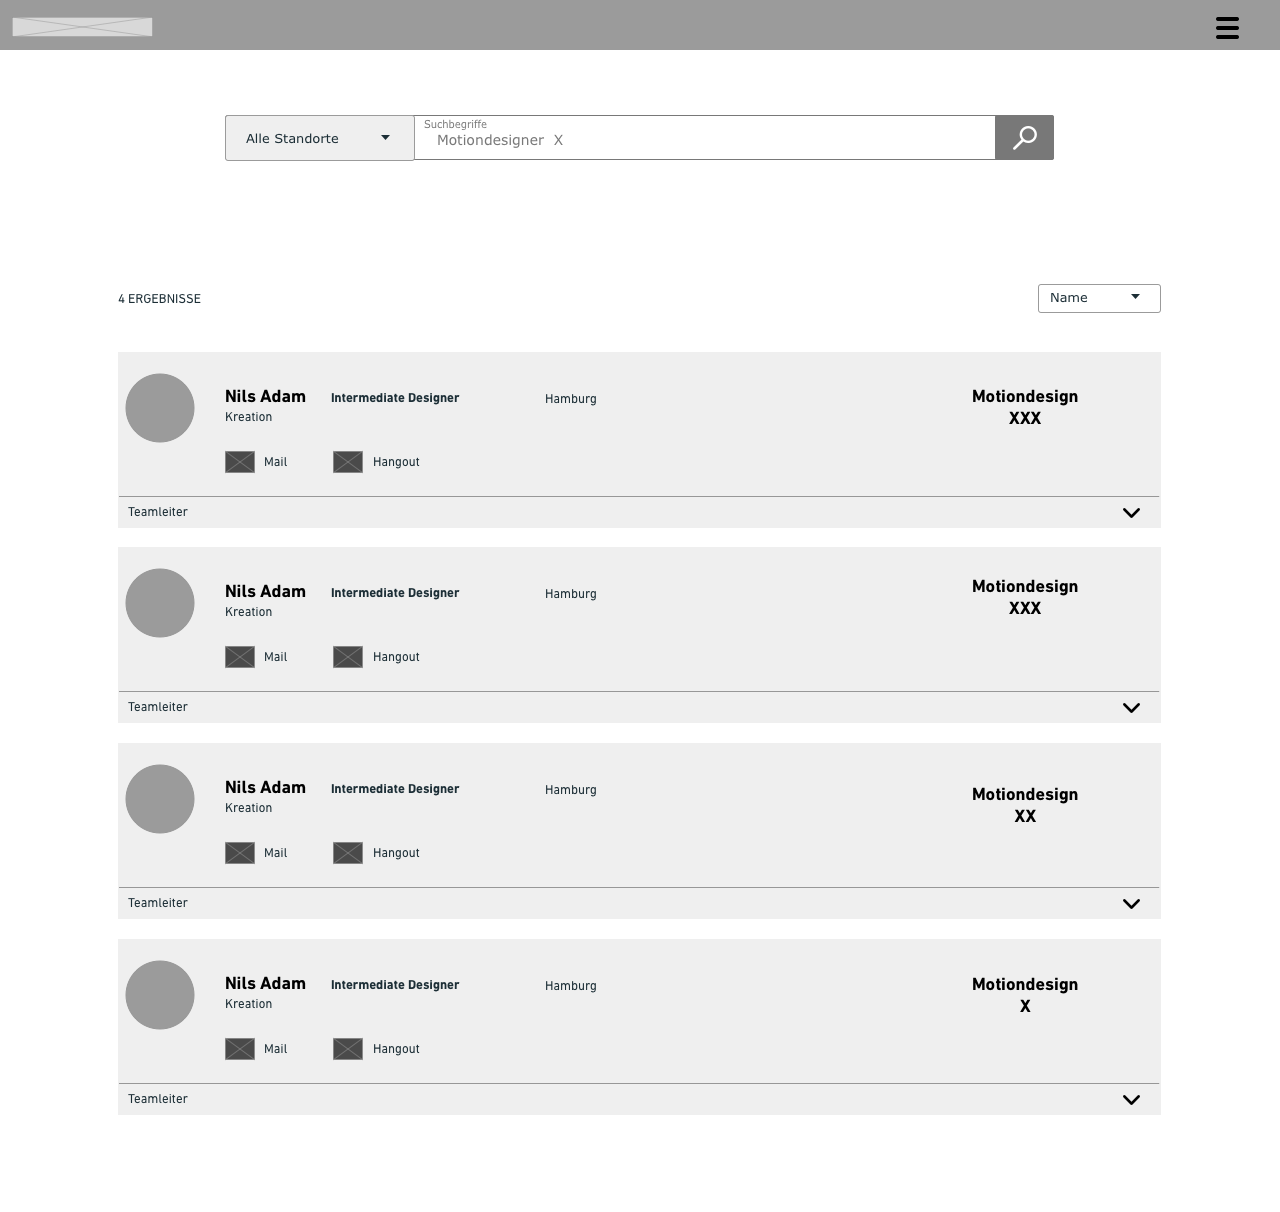
\includegraphics[width=0.8\textwidth]{images/wireframe.png}
    \caption{Wireframe}
    \label{fig:wireframe}
\end{figure}


\section{Requirements}
\subsection{Functional Requirements}
\begin{itemize}
	\item User Profiles
	Anyone can see another user’s profile consisting of basic information about the user such as Name, Location, E-Mail and personal skills. Personal skills are composed of a name, a knowledge level and a will level, both on a scale from one to four.
	\item Employees can provide and edit their skills
	Users can add new skills from a pool of known skills to their own profile. Already added skills can be edited and removed from the profile.
	\item Search
	A search function can be used to find people who have added one or more specific skills to their profile. When searching for multiple skills, only persons matching all of them will will be displayed. The results shall be ordered by knowledge levels and/or wills.
	\item Management of known skills
	New skills can be added to the set of known skills in the application. Existing skills can be edited and removed. Users personal skills are automatically updated when a skill has been edited so that the integrity of the user profiles is maintained at all times.
\end{itemize}



\subsection{Non Functional Requirements}
TODO: Klären und formulieren
\begin{itemize}
	\item Desktop/Devices
	\item Browsers
	\item Scalability
	\item Load/Response Times
\end{itemize}


\section{Commercial Solutions}
